\whiteBGstarBegin
\setcounter{section}{0}
\section{Trắc nghiệm}
\begin{enumerate}[label=\bfseries Câu \arabic*:]
	
	
	\item \mkstar{1}
	
	\cauhoi
	{Điều nào sau đây \textbf{không đúng} khi nói về quan hệ giữa cường độ điện trường và hiệu điện thế?
		\begin{mcq}
			\item Vectơ cường độ điện trường hướng từ nơi có điện thế cao về nơi có điện thế thấp.
			\item Trong một điện trường đều, hiệu điện thế giữa hai điểm này và giữa hai điểm khác có thể bằng nhau.
			\item Hiệu điện thế giữa hai điểm trên cùng một đường sức trong một điện trường đều có thể bằng 0.
			\item Cường độ điện trường tỉ lệ thuận với hiệu điện thế.
		\end{mcq}
		
	}
	\loigiai
	{	\textbf{Đáp án: C.}
	
	}
	\item \mkstar{1}
	
	\cauhoi
	{Cho một điện trường đều có cường độ $E$. Chọn chiều dương cùng chiều với đường sức điện. Gọi $U$ là hiệu điện thế giữa hai điểm M và N trên cùng một đường sức, $d=\overline{\text{MN}}$ là độ dài đại số đoạn MN. Hệ thức nào sau đây đúng?
		\begin{mcq}(4)
			\item $E=\dfrac{U}{2d}$.
			\item $E=\dfrac{U}{d}$.
			\item $E=Ud$.
			\item $E=2Ud$.
		\end{mcq}
		
	}
	\loigiai
	{	\textbf{Đáp án: B.}
	
	}
	\item \mkstar{1}
	
	\cauhoi
	{Trên một đường sức của điện trường đều có hai điểm M và N cách nhau 40 cm. Hiệu điện thế giữa hai điểm M và N là 16 V. Cường độ điện trường có độ lớn là
		\begin{mcq}(4)
			\item 4000 V/m.
			\item 40 V/m.
			\item 400 V/m.
			\item 4 V/m.
		\end{mcq}
		
	}
	\loigiai
	{	\textbf{Đáp án: B.}
		
		Áp dụng công thức:
		$$E=\dfrac{U}{d} = \SI{40}{V/m}.$$
	}
	\item \mkstar{2}
	
	\cauhoi
	{Công của lực điện trường dịch chuyển một điện tích $\SI{-2}{\micro C}$ từ A đến B là 4 mJ. Hiệu điện thế giữa hai điểm A và B là
		\begin{mcq}(4)
			\item 2 V.
			\item 2000 V.
			\item -8 V.
			\item -2000 V.
		\end{mcq}
		
	}
	\loigiai
	{	\textbf{Đáp án: D.}
		
		Áp dụng công thức:
		$$A=qU \Rightarrow U = \SI{-2000}{V}.$$
	}
	\item \mkstar{2}
	
	\cauhoi
	{Hai điểm M và N cùng nằm trên một đường sức của một điện trường đều cách nhau $\SI{2}{m}$. Độ lớn của cường độ điện trường là 500 V/m. Hiệu điện thế giữa hai điểm đó là
		\begin{mcq}(4)
			\item 1000 V.
			\item 125 V.
			\item 2000 V.
			\item 0 V.
		\end{mcq}
		
	}
	\loigiai
	{	\textbf{Đáp án: A.}
		
		Áp dụng công thức:
	$$U=Ed \Rightarrow U = \SI{1000}{V}.$$
	}
	\item \mkstar{2}
	
	\cauhoi
	{Hiệu điện thế giữa hai điểm M và N là $U_\text{MN} = \SI{1}{V}$. Công của lực điện trường làm dịch chuyển điện tích $q=\SI{-1}{\micro C}$ từ M đến N là
		\begin{mcq}(4)
			\item $\SI{-1}{\micro J}$.
			\item $\SI{1}{\micro J}$.
			\item $\SI{-1}{J}$.
			\item $\SI{1}{J}$.
		\end{mcq}
		
	}
	\loigiai
	{	\textbf{Đáp án: A.}
		
		Vì $U_\text{MN} = \SI{1}{V} >0$ nên công của lực điện trường làm dịch chuyển điện tích âm từ M đến N là công cản.
		
		Áp dụng công thức: $A=qU = \SI{-1}{\micro J}$.
	}
	\item \mkstar{2}
	
	\cauhoi
	{Thế năng tĩnh điện của một electron tại điểm M trong điện trường của một điện tích điểm là $\SI{-3.2e-19}{J}$. Điện thế tại điểm M là
		\begin{mcq}(4)
			\item $\SI{3.2}{V}$.
			\item $\SI{-3.2}{V}$.
			\item $\SI{2}{V}$.
			\item $\SI{-2}{V}$.
		\end{mcq}
		
	}
	\loigiai
	{	\textbf{Đáp án: C.}
		
		Áp dụng công thức:
		$$V_\text{M} = \dfrac{A_\text{M}}{q} = \SI{2}{V}.$$
	}
	\item \mkstar{2}
	
	\cauhoi
	{Khi độ lớn điện tích thử đặt tại một điểm tăng lên gấp đôi thì điện thế tại điểm đó
		\begin{mcq}(2)
			\item không đổi.
			\item tăng gấp đôi.
			\item giảm một nửa.
			\item tăng gấp bốn.
		\end{mcq}
		
	}
	\loigiai
	{	\textbf{Đáp án: A.}
		
		Điện thế tại một điểm không phụ thuộc vào độ lớn điện tích thử.
	}
	\item \mkstar{2}
	
	\cauhoi
	{Biết hiệu điện thế giữa hai điểm M, N là $U_\text{MN}=\SI{7}{V}$. Gọi $V_\text{M}$, $V_\text{N}$ lần lượt là điện thế tại M và N. Khẳng định nào sau đây đúng nhất?
		\begin{mcq}(2)
			\item $V_\text{M} = V_\text{N} = \SI{7}{V}$.
			\item $V_\text{M} - V_\text{N} = \SI{7}{V}$.
			\item $V_\text{N} - V_\text{M} = \SI{7}{V}$.
			\item $V_\text{N} + V_\text{M} = \SI{7}{V}$.
		\end{mcq}
		
	}
	\loigiai
	{	\textbf{Đáp án: B.}
		
		Nếu $U_\text{MN} = \SI{7}{V}$ thì có nghĩa là $V_\text{M} - V_\text{N} = \SI{7}{V}$.
	}
	\item \mkstar{2}
	
	\cauhoi
	{Hiệu điện thế giữa hai điểm M, N là 40 V. Chọn câu đúng nhất.
		\begin{mcq}
			\item Điện thế tại M là 40 V, điện thế tại N là 0 V.
			\item Điện thế tại M cao hơn điện thế tại N là 40 V.
			\item Điện thế tại M có giá trị dương, điện thế tại N có giá trị âm.
			\item Điện thế tại N là 40 V, điện thế tại M là 0 V.
		\end{mcq}
		
	}
	\loigiai
	{	\textbf{Đáp án: B.}
		
		Hiệu điện thế giữa hai điểm M, N là $\SI{40}{V}$ thì điện thế tại M cao hơn điện thế tại N là $\SI{40}{V}$.
	}
	\item \mkstar{2}
	
	\cauhoi
	{Mối liên hệ giữa $U_\text{MN}$ và $U_\text{NM}$ là
		\begin{mcq}(4)
			\item $U_\text{MN} = U_\text{NM}$.
			\item $U_\text{MN} = - U_\text{NM}$.
			\item $U_\text{MN} = \dfrac{1}{U_\text{NM}}$.
			\item $U_\text{MN} = -\dfrac{1}{U_\text{NM}}$.
		\end{mcq}
		
	}
	\loigiai
	{	\textbf{Đáp án: B.}
	
	}
	\item \mkstar{2}
	
	\cauhoi
	{Trên một đường sức của một điện trường đều có hai điểm M và N cách nhau 40 cm. Hiệu điện thế giữa hai điểm M và N là 80 V. Cường độ điện trường có độ lớn là
		\begin{mcq}(4)
			\item 2000 V/m.
			\item 2 V/m.
			\item 200 V/m.
			\item 20 V/m.
		\end{mcq}
		
	}
	\loigiai
	{	\textbf{Đáp án: C.}
		
		Áp dụng công thức:
		$$E=\dfrac{U}{d} \Rightarrow E = \SI{200}{V/m}.$$
	}
	\item \mkstar{2}
	
	\cauhoi
	{Giữa hai điểm A và B phải có hiệu điện thế bằng bao nhiêu để một điện tích $q=\SI{1}{\micro C}$ thu được năng lượng $A=\SI{2e-4}{J}$ khi đi giữa hai điểm đó?
		\begin{mcq}(4)
			\item 100 V.
			\item 200 V.
			\item 300 V.
			\item 500 V.
		\end{mcq}
		
	}
	\loigiai
	{	\textbf{Đáp án: B.}
		
		Áp dụng công thức:
		$$A=qU \Rightarrow U = \SI{200}{V}.$$
	}
	\item \mkstar{2}
	
	\cauhoi
	{Hiệu điện thế giữa hai điểm M và N trong một điện trường đều là $U_\text{MN} = \SI{20}{V}$. Một điện tích dịch chuyển cùng chiều điện trường từ M đến N dưới tác dụng của lực điện, với công của lực điện bằng $\SI{1.6e-10}{J}$. Giá trị của điện tích này là
		\begin{mcq}(4)
			\item $q=\SI{6e-6}{C}$.
			\item $q=\SI{6e-9}{C}$.
			\item $q=\SI{8e-12}{C}$.
			\item $q=\SI{8e-15}{C}$.
		\end{mcq}
		
	}
	\loigiai
	{	\textbf{Đáp án: C.}
		
		Áp dụng công thức:
	$$A=qU \Rightarrow q = \SI{8e-12}{C}.$$
	}
	\item \mkstar{2}
	
	\cauhoi
	{Tính công mà lực điện tác dụng lên một electron khi nó chuyển động từ điểm M đến điểm N. Biết hiệu điện thế $U_\text{MN} = \SI{50}{V}$.
		\begin{mcq}(4)
			\item $\SI{8e-18}{J}$.
			\item $\SI{-8e-18}{J}$.
			\item $\SI{3.2e-21}{J}$.
			\item $\SI{-3.2e-21}{J}$.
		\end{mcq}
		
	}
	\loigiai
	{	\textbf{Đáp án: B.}
		
		Áp dụng công thức:
		$$A=qU=\SI{8e-18}{J}.$$
		
		Mà công làm dịch chuyển electron từ M đến N là công âm, nên $A=\SI{-8e-18}{J}$.
	}
	\item \mkstar{3}
	
	\cauhoi
	{Cho 3 điểm M, N, P trong một điện trường đều. Cho $\text{MN} = \SI{3}{cm}$, $\text{NP} = \SI{1}{cm}$, $U_\text{MN} = \SI{3}{V}$, $U_\text{MP} = \SI{1}{V}$. Gọi cường độ điện trường tại M, N, P lần lượt là $E_\text{M}$, $E_\text{N}$, $E_\text{P}$. Kết luận đúng là
		\begin{mcq}(4)
			\item $E_\text{N} > E_\text{M}$.
			\item $E_\text{P} = 2E_\text{N}$.
			\item $E_\text{P} = 3E_\text{N}$.
			\item $E_\text{P} = E_\text{N}$.
		\end{mcq}
		
	}
	\loigiai
	{	\textbf{Đáp án: D.}
		
		Trong một điện trường đều, cường độ điện trường tại mọi điểm bằng nhau.
	}
	\item \mkstar{3}
	
	\cauhoi
	{Trong một điện trường đều, nếu trên một đường sức, giữa hai điểm cách nhau 4 cm có hiệu điện thế 10 V, thì giữa hai điểm cách nhau 6 cm sẽ có hiệu điện thế là
		\begin{mcq}(4)
			\item 8 V.
			\item 10 V.
			\item 15 V.
			\item $\SI{22.5}{V}$.
		\end{mcq}
		
	}
	\loigiai
	{	\textbf{Đáp án: C.}
		
		Ta có:
		$$E=\dfrac{U_1}{d_1} = \dfrac{U_2}{d_2} \Rightarrow U_2 = \dfrac{U_1 d_2}{d_1} = \SI{15}{V}.$$
	}
	\item \mkstar{3}
	
	\cauhoi
	{Một proton bay vào trong điện trường. Lúc proton ở điểm A thì tốc độ của nó là $\SI{2.5e4}{m/s}$. Khi bay đến B tốc độ của proton bằng 0. Điện thế tại A bằng $\SI{500}{V}$, điện thế tại B gần giá trị nào nhất sau đây? Cho biết proton có khối lượng $\SI{1.67e-27}{kg}$ và có điện tích $\SI{1.6e-19}{C}$.
		\begin{mcq}(4)
			\item $\SI{403.3}{V}$.
			\item $\SI{503.3}{V}$.
			\item $\SI{703.3}{V}$.
			\item $\SI{603.3}{V}$.
		\end{mcq}
		
	}
	\loigiai
	{	\textbf{Đáp án: B.}
		
		Áp dụng định lý động năng cho chuyển động của proton từ điểm A đến điểm B:
		$$W_\text{đ B} - W_\text{đ A} = qU_\text{AB} \Rightarrow U_\text{AB} = \SI{-3.26}{V}.$$
		
		Mà $U_\text{AB} = V_\text{A} - V_\text{B} \Rightarrow V_\text{B} \approx \SI{503.3}{V}$.
	}
	\item \mkstar{3}
	
	\cauhoi
	{Một electron bay với vận tốc $\SI{1.2e7}{m/s}$ từ một điểm có điện thế $V_1=\SI{600}{V}$ dọc theo hướng các đường sức của một điện trường đều. Biết điện tích của electron là $\SI{-1.6e-19}{C}$ và khối lượng của nó là $\SI{9.1e-31}{kg}$. Điện thế $V_2$ tại điểm mà ở đó electron dừng lại là
		\begin{mcq}(4)
			\item $\SI{150.4}{V}$.
			\item $\SI{170.5}{V}$.
			\item $\SI{190.5}{V}$.
			\item $\SI{200}{V}$.
		\end{mcq}
		
	}
	\loigiai
	{	\textbf{Đáp án: C.}
		
		Áp dụng định lý động năng:
		$$W_\text{đ 2} - W_\text{đ 1} = A \Leftrightarrow -\dfrac{mv^2}{2} = q(V_1 - V_2) \Rightarrow V_2 = \SI{190.5}{V}.$$
	}
	\item \mkstar{4}
	
	\cauhoi
	{Cho ba bản kim loại phẳng tích điện 1, 2, 3 đặt song song lần lượt cách nhau những khoảng $d_{12} = \SI{5}{cm}$, $d_{23} = \SI{8}{cm}$. Bản 1 và 3 tích điện dương, bản 2 tích điện âm. Biết $E_{12}=\SI{4e4}{V/m}$, $E_{23} = \SI{5e4}{V/m}$. Tính điện thế $V_2$, $V_3$ của các bản 2 và 3 nếu lấy gốc điện thế ở bản 1 ($V_1=0$).
		\begin{mcq}(2)
			\item $V_2=\SI{2000}{V}$, $V_3=\SI{-2000}{V}$.
			\item $V_2\SI{2000}{V}$, $V_3=\SI{4000}{V}$.
			\item $V_2=\SI{-2000}{V}$, $V_3=\SI{4000}{V}$.
			\item $V_2=\SI{-2000}{V}$, $V_3=\SI{2000}{V}$.
		\end{mcq}
		
	}
	\loigiai
	{	\textbf{Đáp án: D.}
		
		Ta có:
		$$U_{12} = E_{12} d_{12} = \SI{2000}{V};$$
		$$U_{32} = E_{32} d_{32} = \SI{4000}{V}.$$
		
		Vì bản 1 và 3 tích điện dương, bản 2 tích điện âm nên khi chọn $V_1=0$ thì
		$$U_{12} = V_1 - V_2 \Rightarrow V_2 = \SI{-2000}{V}.$$
		$$U_{32} = V_3 - V_2 \Rightarrow V_3 = \SI{2000}{V}.$$
	}
\end{enumerate}

\whiteBGstarEnd

\loigiai
{
	\begin{center}
		\textbf{BẢNG ĐÁP ÁN}
	\end{center}
	\begin{center}
		\begin{tabular}{|m{2.8em}|m{2.8em}|m{2.8em}|m{2.8em}|m{2.8em}|m{2.8em}|m{2.8em}|m{2.8em}|m{2.8em}|m{2.8em}|}
			\hline
			1.C  & 2.B  & 3.B  & 4.D  & 5.A  & 6.A  & 7.C  & 8.A  & 9.B  & 10.B  \\
			\hline
			11.B  & 12.C  & 13.B  & 14.C  & 15.B  & 16.D  & 17.C  & 18.B  & 19.C  & 20.D  \\
			\hline
		\end{tabular}
	\end{center}
}
\section{Tự luận}
\begin{enumerate}[label=\bfseries Câu \arabic*:]
	\item \mkstar{1}
	
	\cauhoi{
		Điện thế tại một điểm là gì? Hiệu điện thế giữa hai điểm trong điện trường là gì? Nêu công thức định nghĩa hai đại lượng trên.
	}
	
	\loigiai{
		
		Điện thế tại một điểm M trong điện trường là đại lượng đặc trưng cho điện trường về phương diện tạo ra thế năng khi đặt tại đó một điện tích $q$.
		
		Công thức:
		$$V_\text{M} = \dfrac{A}{Q}.$$
		
		Hiệu điện thế giữa hai điểm trong điện trường là đại lượng đặc trưng cho khả năng thực hiện công của điện trường khi có 1 điện tích di chuyển giữa hai điểm đó.
		
		Công thức:
		$$U_\text{MN} = V_\text{M} - V_\text{N} = \dfrac{A_\text{MN}}{q}.$$
	}
	
	\item \mkstar{2}
	
	\cauhoi{
		Khi bay từ điểm M đến điểm N trong điện trường, electron tăng tốc, động năng tăng thêm $\SI{250}{eV}$. Biết rằng $\SI{1}{eV} = \SI{1.6e-19}{J}$, xác định $U_\text{MN}$.
	}
	
	\loigiai{
		Áp dụng định lý động năng:
		$$A=W_\text{đ 2} - W_\text{đ 1} = \SI{4e-17}{J}.$$
		
		Hiệu điện thế:
		$$U_\text{MN} = \dfrac{A}{q} = \SI{-250}{V}.$$
		
	}
	\item \mkstar{3}
	
	\cauhoi{
		Bắn một electron (tích điện $-|e|$ và khối lượng $m$) với vận tốc $v_0$ vào điện trường đều giữa hai bản kim loại phẳng theo phương song song, cách đều hai bản kim loại (xem hình vẽ).
		\begin{center}
			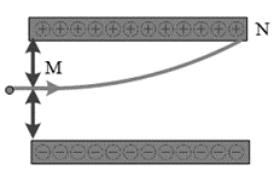
\includegraphics{../figs/VN11-2021-PH-TP006-1}
		\end{center}
	
	Hiệu điện thế giữa hai bản là 200 V. Biết rằng electron bay ra khỏi điện trường tại điểm nằm sát mép một bản. Công của lực điện trong sự dịch chuyển của electron trong điện trường là bao nhiêu?
	}
	
	\loigiai{
	Công của lực điện:
	$$A_\text{MN} = qU_\text{MN} = -|e| \dfrac{-U}{2} = \SI{0.5}{} |e| U = \SI{1.6e-17}{J}.$$	
		
	}
	\item \mkstar{4}
	
	\cauhoi{
		Một quả cầu khối lượng $\SI{4.5e-3}{kg}$ treo vào một sợi dây cách điện dài 1 m. Quả cầu nằm giữa hai tấm kim loại song song, thẳng đứng như hình vẽ.
		\begin{center}
			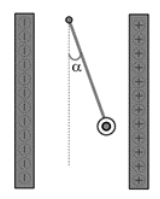
\includegraphics{../figs/VN11-2021-PH-TP006-2}
		\end{center}
	
	Hai tấm cách nhau 4 cm. Đặt một hiệu điện thế 75 V vào hai tấm đó thì quả cầu lệch ra khỏi vị trí ban đầu 1 cm. Lấy $g=\SI{10}{m/s^2}$. Tính độ lớn điện tích của quả cầu.
	}
	
	\loigiai{
		\begin{center}
			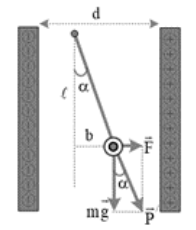
\includegraphics{../figs/VN11-2021-PH-TP006-4}
		\end{center}
		
		Quả cầu lệch về bản dương nên nó tích điện âm. Khi hệ cân bằng thì
		$$\tan \alpha = \dfrac{b}{l} = \dfrac{F}{mg} = \dfrac{|q|E}{mg} = \dfrac{|q|U}{mgd} \Rightarrow |q| = \dfrac{mgd}{U} \cdot \dfrac{b}{l} = \SI{2.4e-7}{C}.$$
	}
	\item \mkstar{4}
	
	\cauhoi{
		Ba điểm A, B, C tạo thành tam giác vuông tại A đặt trong điện trường đều có vectơ cường độ điện trường song song với AB. Cho $\alpha =60^\circ$, $\text{BC} = \SI{10}{cm}$ và $U_\text{BC} = \SI{400}{V}$. Tính $U_\text{AC}$, $U_\text{BA}$ và $E$.
		\begin{center}
			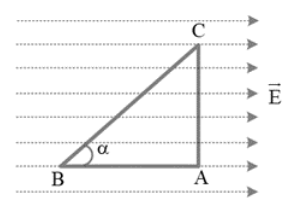
\includegraphics{../figs/VN11-2021-PH-TP006-3}
		\end{center}
	}
	
	\loigiai{
		Cường độ điện trường:
		$$U_\text{BC} = E \cdot \text{BC} \cdot \cos \alpha \Rightarrow E = \SI{8000}{V/m}.$$
		
		Hiệu điện thế $U_\text{AC}$:
		$$U_\text{AC} = E \cdot \text{AC} \cdot \cos 90^\circ = 0.$$
		
		Hiệu điện thế $U_\text{BA}$:
		$$U_\text{BA} = U_\text{BC} + U_\text{CA} = \SI{400}{V}.$$
	}
	
\end{enumerate}